\documentclass[a4,10pt]{article} \usepackage[pdftex]{graphicx}
\usepackage{setspace}
%\usepackage{lineno}
\usepackage{color}
\usepackage{hyperref}
\hypersetup{
    colorlinks,%
    citecolor=black,%
    filecolor=black,%
    linkcolor=black,%
    urlcolor=blue
}
\definecolor{PiranaOrange}{rgb}{0.9,0.4,0.1}
\definecolor{Blue}{rgb}{0.0,0.0,0.7}
\definecolor{Red}{rgb}{0.7,0.0,0.0}
\definecolor{Grey}{rgb}{0.2,0.2,0.2}
\definecolor{grey2}{rgb}{.92, .92, .92}

\pdfinfo{
   /Author (Ron Keizer, Coen van Hasselt, Pirana Software & Consulting BV)
   /Title  (Pirana Quick Guide)
}

\bibliographystyle{unsrt}%Choose a bibliograhpic style}
%\usepackage{utopia} %\usepackage{charter} %\usepackage{palatino}
%\usepackage{bookman} %\usepackage{newcent} %\usepackage{times}
%\usepackage[options]{natbib} \sloppy
\renewcommand{\familydefault}{\sfdefault} 
\renewcommand{\emph}[1]{\textbf{\textcolor{Grey}{#1}}} 
\oddsidemargin 1cm
\textwidth 14cm
\textheight 20cm

\begin{document}

{\centering
  \vspace{-100pt}
  \textbf{
    \textcolor{PiranaOrange}{\Large Pirana}
  }\\
  \vspace{5pt} \scriptsize \textcolor{Grey}{The flexible modeling
    environment for NONMEM} \\ \normalsize
  \vspace{12pt}
  \hspace{5pt}
\includegraphics[scale=0.14]{images/pirana_logo.jpg}\\
  \vspace{18pt}

  {\large
    \emph{Quick Guide: Xpose graphics using Pirana}  \vspace{10pt} \\
        Version 1.1
  }

}
\vspace{25pt}

\begin{center}
   {\colorbox{grey2}{
         \begin{minipage}[t]{0.9\textwidth}
\subsubsection*{Scope}
This Pirana Quick Guide explains how to use Pirana to generate
diagnostic graphs using Xpose. Please note that a separate Quick Guide
describes how to create VPCs in PsN / Xpose.
          \end{minipage}
      }
   }
\end{center}

\subsubsection*{Generating appropriate NONMEM output tables for Xpose}
\begin{itemize}
\item Before Xpose diagnostic graphics can be generated, the model
  first needs to be executed while generating output tables in a
  specific format and naming.
\item Briefly, for a controlstream named run10.mod, output tables such
  as sdtab10 (observations/predictions), patab10 (parameters), cotab10
  (continuous covariates), and catab10 (categorical covariates) should
  be generated, with the NOPRINT and ONEHEADER options.
\item For more information on how to generate Xpose-ready \$TABLE
  output files, please refer to
  \href{'http://xpose.sourceforge.net/manual.pdf''}{the Xpose manual}.
\end{itemize}

\subsubsection*{Generating Xpose graphs using the integrated Pirana menu}
\begin{itemize}
\item Select the preferred run and select Xpose from the right
  mouse-button menu, and subsequently 'Run Xpose commands' (Figure
  \ref{fig:Fig1}).
\begin{figure}[h] \centering
    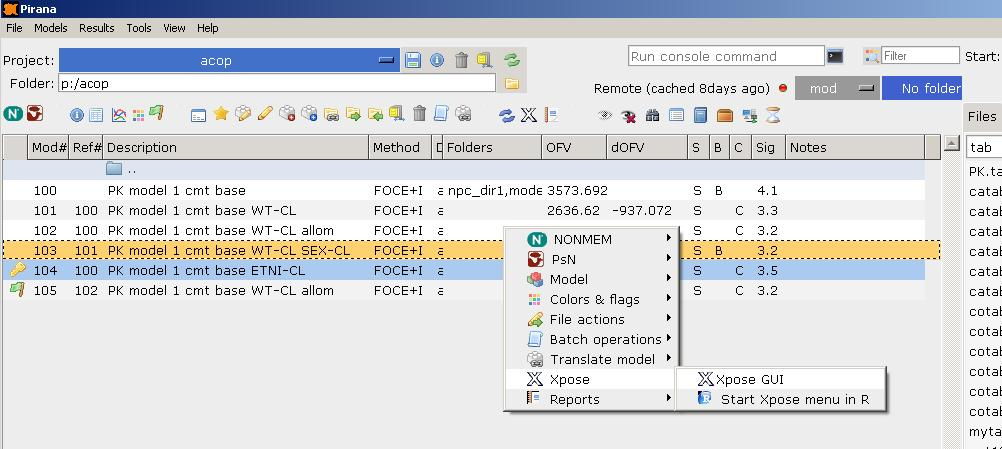
\includegraphics[scale=.32]{images/xpose_1.JPG}
    \caption{Selecting a run and executing the Rub Xpose commands winow\label{fig:Fig1}}
\end{figure}
\item In the dialog window that is opened, different Xpose graphs may
  be selected and defined (Figure \ref{fig:Fig2}).
\begin{figure}[h] \centering
    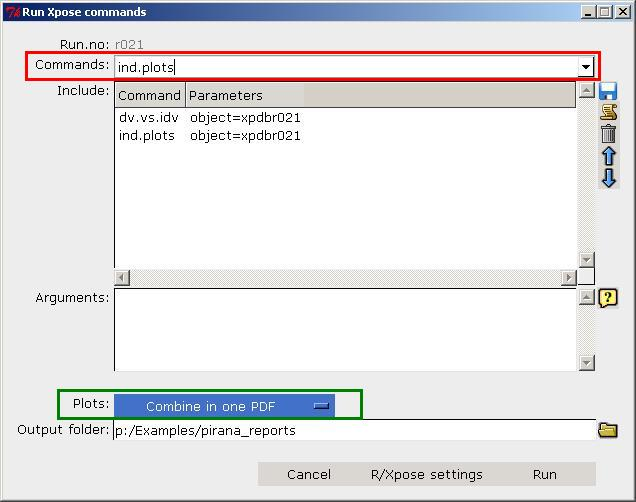
\includegraphics[scale=.45]{images/xpose_2.jpg}
    \caption{Run Xpose commands window\label{fig:Fig2}}
\end{figure}
\item From the \emph{Commands menu} (red square), \emph{multiple}
  Xpose plots may be added to the included list of Xpose plots.
\item Additional \emph{Arguments} may be specified for each Xpose
  command. A reference to possible arguments is provided under the
  \emph{\Large{?}} sign.
\item Several options are available for the output format of the
  \emph{Plots}. The easiest option is to automatically generate the
  graph and save as PDF (default) or PNG file.
\item If multiple Xpose graphs are selected, these will be appended in
  the output file (except PNG).
\item Alternative output formats of the plots are to generate the
  R-code only, or to to generate Sweave code for LaTeX documents.
\item If all settings have been configured, the plot(s) may be
  generated by pressing the execute button (\emph{\Large{$>$}}).
\item If output was directed to a PDF file, the PDF will be opened automatically
  once it is generated (Figure \label{fig:Fig3}).
\begin{figure}[h] \centering
    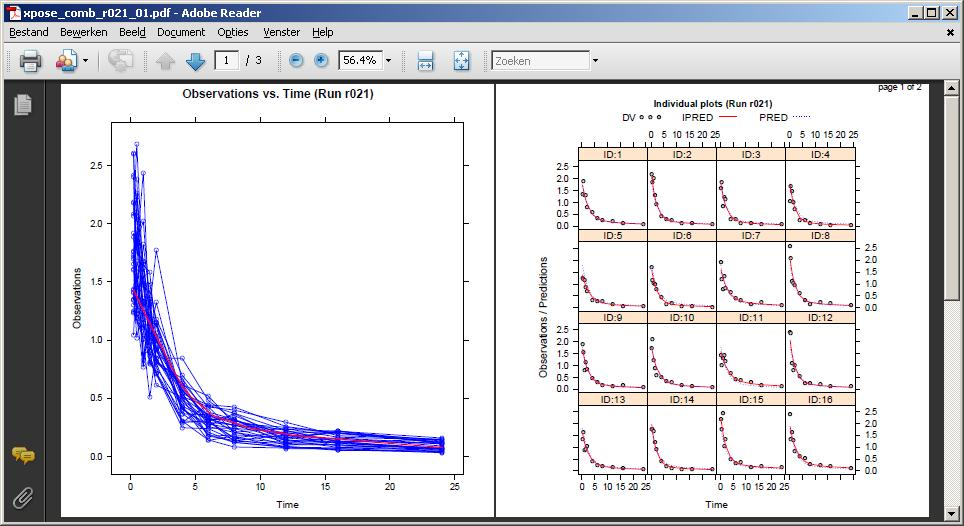
\includegraphics[scale=.4]{images/xpose_3.jpg}
    \caption{Xpose graphs in output PDF file\label{fig:Fig3}}
\end{figure}
\item Lists of commands can be saved and loaded from this dialog as
  well. This can be useful e.g. for standardized report generation.
\end{itemize}

\subsubsection*{Generating Xpose graphs using the conventional menu in R}
\begin{itemize}
\item Alternatively, it is possible to automatically open the
  text-based Xpose menu in R from within Pirana.
\item Select the preferred run and select Xpose from the right
  mouse-button menu, and subsequently ' Start Xpose menu' (Figure 1).
\item The Xpose menu will now be started in R and the associated table
  files will be loaded into Xpose, from where graphs may be generated.
\end{itemize}


\end{document}
